\begin{figure*}[ht]
    \centering
    \begin{minipage}[t]{0.32\textwidth}
        \centering
        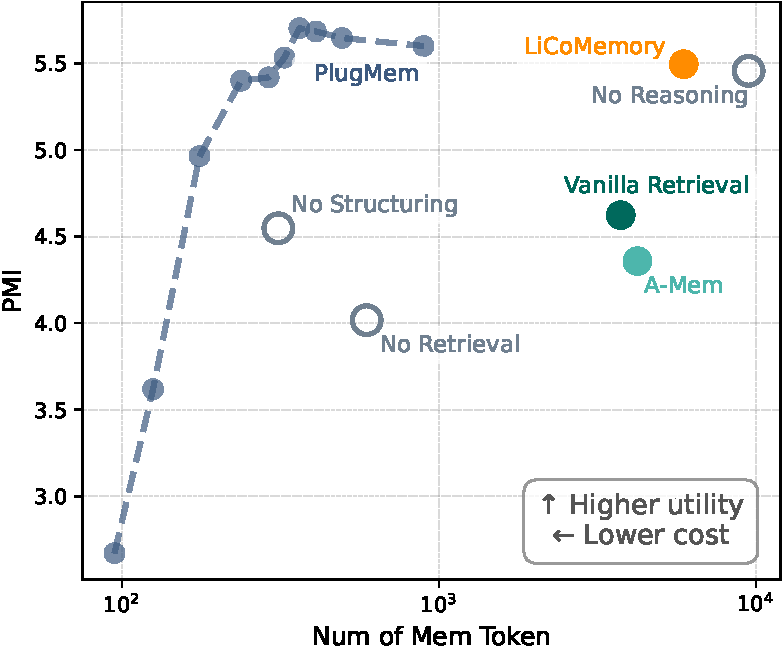
\includegraphics[width=\linewidth]{Figures/PMI_LME.pdf}
        {\small LongMemEval}
    \end{minipage}
    \hfill
    \begin{minipage}[t]{0.332\textwidth}
        \centering       
        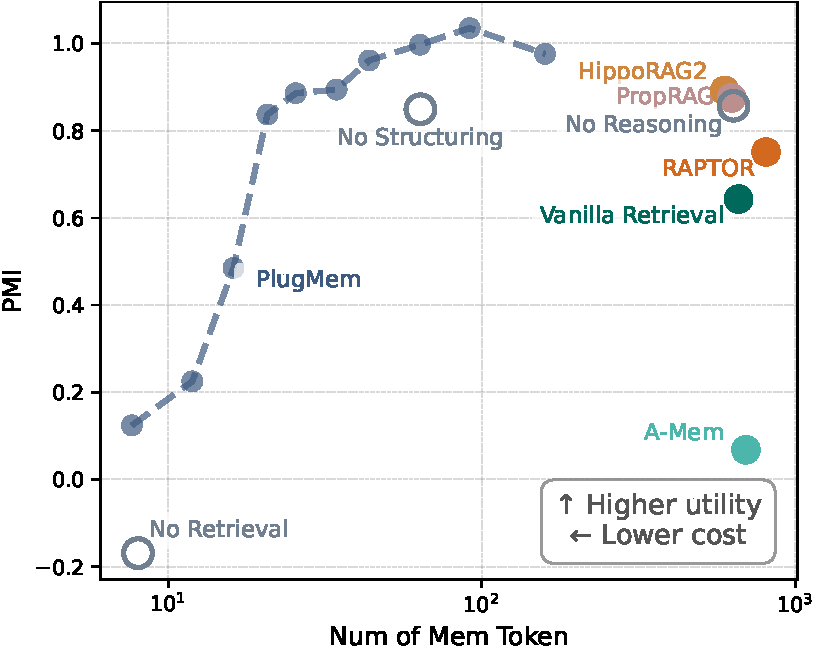
\includegraphics[width=\linewidth]{Figures/PMI_HotPotQA.pdf}
        {\small HotpotQA}
    \end{minipage}
    \hfill
    \begin{minipage}[t]{0.325\textwidth}
        \centering
        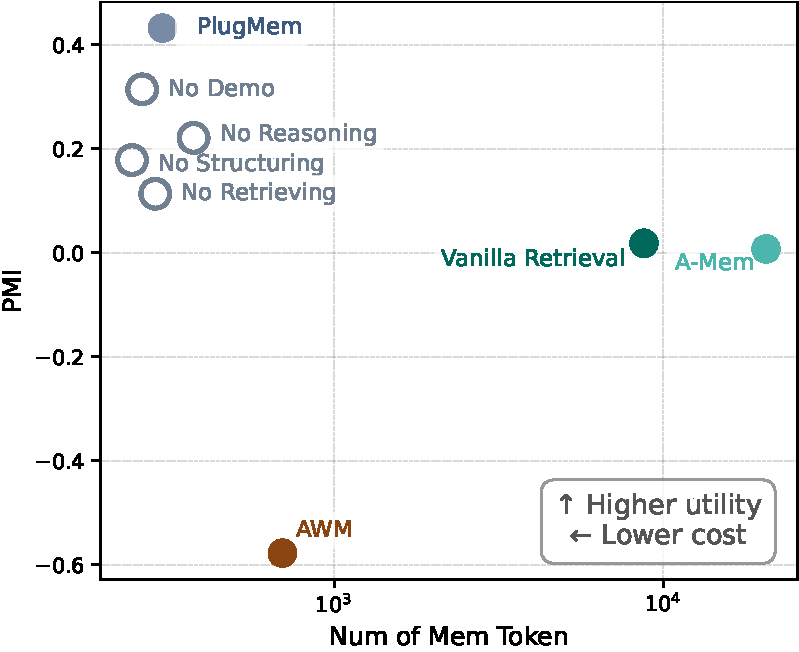
\includegraphics[width=\linewidth]{Figures/PMI_WebArena.pdf}
        {\small WebArena}
    \end{minipage}
    \caption{\label{fig:utility_cost}
    Utility–cost analysis across benchmarks. Each point represents a memory method, with the x-axis indicating agent-side memory cost (in tokens) and the y-axis indicating decision-relevant utility (in bits). The slope of the line connecting a point to the origin corresponds to information density (bit per token). Curves are obtained by sweeping the memory token budget on a randomly sampled subset of benchmark tasks, illustrating how memory utility initially increases with budget, then saturates, and may eventually decline as additional memory becomes counterproductive, for example by introducing noise or interference in decision-making. \textbf{\plugmem consistently achieves a more favorable utility–cost trade-off, dominating prior approaches by providing higher decision-relevant utility under smaller memory budgets across benchmarks.}
    }
\end{figure*}

\section{Experiments}
\label{sec:experiments}
\subsection{Evaluation Framework}
\label{sec:4.1}
We evaluate \plugmem using standard benchmark-wise metrics (e.g., accuracy, F1-score, success rate, etc.) to measure end-task performance.
However, such metrics alone are insufficient for evaluating agentic memory, as they fail to capture the trade-off between decision-relevant utility and agent-side cost.
We therefore propose an information-theoretic measure that quantifies the \emph{decision-relevant information gain per memory token} contributed by the memory module.
Specifically, for each decision instance with state $s$ and gold optimal action $a^{*}$, let the base agent’s prior belief be $P_{\text{base}}(a^{*}\mid s)$ and the memory-augmented posterior be $P_{\text{mem}}(a^{*}\mid s,m)$ after consuming memory $m$.
We define the \emph{Decision Information Gain} as point-wise mutual information (PMI):
\begin{equation}
\label{eq:pmi}
\mathrm{PMI}(a^{*}; m \mid s)=\log_{2}\frac{P_{\text{mem}}(a^{*}\mid s,m)}{P_{\text{base}}(a^{*}\mid s)}
\end{equation}
%
and normalize by memory length $|m|$ (in tokens) to obtain \emph{Memory Information Density} (bits / token):
\begin{equation}
\label{eq:density_single}
\rho(a^{*},m)=\frac{\mathrm{PMI}(a^{*}; m \mid s)}{|m|} %.
\end{equation}
%
Over a dataset, we report a global, amortized density via a ratio-of-sums:
\begin{equation}
\label{eq:density_global}
\rho_{\text{global}}=\frac{\sum_{i}\mathrm{PMI}(a^{*}_{i}; m_{i}\mid s_{i})}{\sum_{i}|m_{i}|} %.
\end{equation}

Measured in bits per token, our metric is task-agnostic and thus comparable across tasks. Cross-task variation in its magnitude reflects a utility–cost trade-off: higher density arises when memory yields larger decision-relevant gains or does so with fewer tokens, while lower density occurs when the base agent already solves the task well or when useful memory must be expressed verbosely. Appendix~\ref{app:memory_information_density} details the complete analysis framework and additional components beyond the main-text description.

\subsection{Common Experimental Setup}

We evaluate \plugmem unchanged across three heterogeneous benchmarks that stress different aspects of agentic memory: 
\textit{i)} LongMemEval~\citep{wu2024longmemeval} for long-horizon conversational memory,
\textit{ii)} HotpotQA~\citep{yang2018hotpotqadatasetdiverseexplainable} for multi-hop knowledge retrieval and reasoning, and 
\textit{iii)} WebArena~\citep{zhou2024webarenarealisticwebenvironment} for interactive web-based decision-making.

Across all benchmarks, we adopt a unified memory evaluation protocol to ensure fair comparison.
Unless otherwise specified, we use NV-Embed-v2~\citep{lee2025nvembedimprovedtechniquestraining} for embedding-based retrieval.
Retrieval is performed under a fixed budget (e.g., top-K retrieval), which is held constant across methods within each benchmark.
For \plugmem, the structuring and reasoning modules are instantiated using Qwen2.5-32B/72B-Instruct~\citep{qwen2025qwen25technicalreport} and GPT-4o~\citep{openai2024gpt4o}, while all base agents are driven by the same model unless explicitly stated.
Decoding parameters are fixed across methods to eliminate confounding effects.
For WebArena, we distinguish between online and offline evaluation phases to assess knowledge transfer and reuse; the detailed experimental design is described in Section~\ref{subsec:knowledge_transfer}.

Baselines are grouped into three categories:
\textit{i)} Vanilla, which do not rely on external memory;
\textit{ii)} Task-agnostic, which employ generic retrieval or agentic memory mechanisms not tailored to the benchmark;
and \textit{iii)} Task-specific, which incorporate benchmark-specific memory representations or retrieval heuristics.

Detailed benchmark-specific settings, prompt templates, and benchmark-level analysis are provided in Appendix~\ref{app:add_exp_details}.

\begin{table}[t!]
\centering
\caption{Results on LongMemEval.
$\text{\#Tok}_{\text{Avg.}}$ is the average length of memory tokens.
Experiments use NV-Embed-v2 (abbreviated as NVE) as the embedding model for retrieval, and Qwen2.5-32B (Q32) / Qwen2.5-72B (Q72) / gpt-4o (4o) as base LLMs for structuring and reasoning. 
* denotes results taken from previous work. 
$\dagger$ denotes methods evaluated on a subset of the full benchmark. Best is \textbf{bolded}.}
\label{tab:longmemeval_res_main}

\begin{threeparttable}
\resizebox{0.48\textwidth}{!}{
\begin{tabular}{c|cc|c|cc}
\toprule
Method & Emb & LLM & Acc. & $\text{\#Tok}_{\text{Avg.}}$ & Info. Density\\
\rowcolor{groupgray}\multicolumn{6}{c}{Vanilla Baseline}          \\
No Context & - & Q72 & 14.8 & - & -\\
All Context & - & Q72 & 62.4 & 107K & 4.2e-5  \\
\rowcolor{groupgray}\multicolumn{6}{c}{Task-Agnostic}          \\
Vanilla Retrieval & NVE & Q72 & 63.6 & 3742.52 & 1.2e-3\\
A-Mem$^{\dagger}$ & NVE & 4o + Q72 & 61.0 & 4225.85 & 1.0e-3 \\
\rowcolor{groupgray}\multicolumn{6}{c}{Task-Specific}          \\
Zep* & BGE-m3 & 4o & 71.2 & 1600 & - \\
LiCoMemory$^{\dagger}$ & NVE & 4o + Q72 & 73.0 & 5914.85 & 9.3e-4 \\
\rowcolor{ShadowBlue}\multicolumn{6}{c}{Ours}          \\
\plugmem & NVE & Q32 + Q72 & \textbf{75.1} & \textbf{362.58} &  \textbf{1.6e-2}\\
\bottomrule
\end{tabular}
}

\begin{tablenotes}[flushleft]
\scriptsize
\item \parbox{0.5\textwidth}{\textit{Note.} More abbreviations: 
Llama3.3-70B (L70).}
\end{tablenotes}
\end{threeparttable}
\end{table}

\begin{table}[t!]
\centering
\caption{Results on HotpotQA. EM means Exact Match.
* denotes results taken from previous work. 
We \underline{underline} the upper bound performance and \textbf{bold} the best.}
\label{tab:hotpotqa_res_main}
\resizebox{0.48\textwidth}{!}{
\begin{tabular}{c|cc|cc|c|c}
\toprule
Mem. Method      & Emb & LLM & EM & F1 & $\text{\#Tok}_{\text{Avg.}}$ &  Info. Density\\
\rowcolor{groupgray}\multicolumn{7}{c}{Vanilla Baseline}          \\
No Context   & - & Q32 & 22.1 & 31.0 & - &  - \\
Gold Context & - & Q32 & \underline{69.2} & \underline{82.1} & 86.5 &  \underline{1.6e-1} \\
\rowcolor{groupgray}\multicolumn{7}{c}{Task-Agnostic}          \\
Vanilla Retrieval & NVE & Q32  & 51.7 & 62.7 & 659.2 & 1.2e-2 \\
A-Mem       & NVE & Q32 & 43.8 & 53.6 & 695.6 & 1.2e-2     \\
\rowcolor{groupgray}\multicolumn{7}{c}{Task-Specific}          \\
GraphRAG*   & NVE & L70 & 55.2 & 68.6 & - & -   \\
RAPTOR      & NVE & Q32 & 56.7 & 69.7 & 806.3 &  1.1e-2     \\
PropRAG     & NVE & Q32 & 57.8 & 72.1 & 626.1 & 1.9e-2    \\
HippoRAG2   & NVE & Q32 & 60.0 & 73.3 & 595.1 & 1.9e-2       \\
\rowcolor{ShadowBlue}\multicolumn{7}{c}{Ours}                   \\
\plugmem         & NVE & Q32 & \textbf{61.4} & \textbf{74.1} & \textbf{81.6} & \textbf{1.4e-1}  \\
\bottomrule
\end{tabular}
}
\end{table}

\begin{table}[t!]
\centering
\caption{Results on WebArena. SR means Success Rate. Each site-domain is split into (online/offline) sets. Shopping contains (38/149) tasks, GitLab contains (37/143), and Multi-set contains (10/38). * denotes results taken from previous work. AWM does not natively support Multi-site tasks. Best SR is \textbf{bolded}.}
\label{tab:webarena-main}
\resizebox{0.48\textwidth}{!}{
\begin{tabular}{c|cc|ccc|cc}
\toprule
 &  &  & \multicolumn{3}{c|}{SR \% (on/off)} & \\
\cmidrule(lr){4-6}
Method & Emb & Agent 
& Shopping  
& GitLab
& Multi-site

& $\text{\#Tok}_{\text{Avg.}}$

& Info. Density \\

\rowcolor{groupgray}\multicolumn{8}{c}{Vanilla Baseline} \\

AgentOccam*  & -   & 4o   & 42.1/43.6 & 37.8/39.2 & \textbf{20.0}/15.8 & - & - \\

\rowcolor{groupgray}\multicolumn{8}{c}{Task-Agnostic} \\

Van. Retrieval & NVE & Q32+4o  & 43.0 /42.3& 40.5/41.3 & 10.0/18.4 & 8733 & 2.0e-6\\
A-Mem & NVE & Q32+4o & 44.7/44.3 & 37.8/38.5 & \textbf{20.0}/15.8 & 20516 & 3.4e-7\\

\rowcolor{groupgray}\multicolumn{8}{c}{Task-Specific} \\

AWM & - & 4o & 26.3/28.2 & 27.0/27.3 & - & 696 & -7.9e-4 \\

\rowcolor{ShadowBlue}\multicolumn{8}{c}{Ours} \\

\plugmem & NVE & Q32+4o & \textbf{52.6}\textbf{/58.4} & \textbf{51.4}\textbf{/55.2}  & \textbf{20.0}\textbf{/21.6} & \textbf{301} & \textbf{1.4e-3}\\
\bottomrule
\end{tabular}
}
\end{table}

\subsection{RQ1: Does \plugmem Improve Performance and Memory Efficiency Across Tasks?}
Our first research question examines whether a single, task-agnostic memory module can consistently improve agent performance while reducing memory consumption across heterogeneous tasks.
Results on LongMemEval, HotpotQA, and WebArena (Tables~\ref{tab:longmemeval_res_main}, \ref{tab:hotpotqa_res_main}, \ref{tab:webarena-main}) show a consistent pattern despite large differences in task structure and interaction modality.
First, \plugmem improves end-task performance over both task-agnostic and task-specific baselines.
Second, these gains are achieved with substantially fewer memory tokens injected into the agent context. 
Thus, \plugmem attains the highest \emph{information-gain density} under the unified information-theoretic analysis introduced in Section~\ref{sec:4.1}.
This trade-off is further illustrated by the utility–cost visualization in Figure~\ref{fig:utility_cost}, where \plugmem consistently shifts toward higher utility and lower agent-side cost across all three benchmarks.

The results indicate that \plugmem retrieves \emph{more decision-relevant memory}.
By abstracting raw experience into compact propositional and prescriptive knowledge, the memory module provides higher utility per token, enabling the base agent to reason more effectively under tight context budgets.

\subsection{RQ2: What Is the Role of Each Component in \plugmem?}

We next analyze the contribution of each component in \plugmem via ablations on all benchmarks (Tables~\ref{tab:longmemeval_ablation}, \ref{tab:hotpotqa_ablation}, \ref{tab:webarena_ablation}).
Removing retrieval leads to the most severe performance degradation across tasks, underscoring that memory is \textit{only} useful when relevant experience can be accessed at decision time.
However, this does not imply that retrieval alone drives performance gains.
Rather, retrieval determines whether memory is operative at all, while its effectiveness is bounded by how memory is represented.
The structuring module improves retrieval by organizing memory at appropriate abstraction levels, allowing the retriever to more effectively identify and access task-relevant knowledge.
The reasoning module plays a complementary role, primarily affecting memory efficiency by controlling how retrieved knowledge is compressed and consumed.

Overall, retrieval determines \emph{whether} memory helps, structuring determines \emph{what} can be retrieved, and reasoning determines \emph{how efficiently} retrieved memory can be used.
Retrieval thus constitutes the defining bottleneck, while structuring and reasoning modulate effectiveness and efficiency once retrieval is in place.
\begin{table}[t!]
\centering
\caption{Ablation study on LongMemEval.}
\label{tab:longmemeval_ablation}
\resizebox{0.48\textwidth}{!}{
\begin{tabular}{c|cc|c|cc}
\toprule
Method & Emb & LLM & Acc. & $\text{\#Tok}_{\text{Avg.}}$ & Info. Density\\
\midrule
\rowcolor{ShadowBlue}
\plugmem & NVE & Q32 + Q72 & \textbf{75.1} & 362.58 & \textbf{1.6e-2} \\
\specialrule{0.6pt}{0pt}{2pt}
No Structuring & NVE & Q32 + Q72 & 62.8 & \textbf{311.12} & 1.4e-2\\
No Retrieval & - & Q32 + Q72 & 57.2 & 591.2 & 6.8e-3\\
No Reasoning & NVE & Q32  & 72.4 & 9478.59 & 5.8e-4 \\
\bottomrule
\end{tabular}
}
\end{table}
%\\
\begin{table}[t]
\centering

\caption{Ablation study on HotpotQA.}
\label{tab:hotpotqa_ablation}
\begin{threeparttable}
\resizebox{0.48\textwidth}{!}{
\begin{tabular}{c|cc|cc|c|c}
\toprule
Method     & Emb & LLM & EM & F1 & $\text{\#Tok}_{\text{Avg.}}$ & Info. Density\\
\midrule
\rowcolor{ShadowBlue}
\plugmem       & NVE   & Q32 & \textbf{61.4} & \textbf{74.1} & \textbf{81.6} & \textbf{1.4e-1}  \\
\specialrule{0.6pt}{0pt}{2pt}
 No Structuring & NVE & Q32 & 51.4 & 62.0 & 116.7 & 6.8e-2  \\
 No Retrieval & -  & Q32 & 20.0  & 24.3  & 8.0\tnote{1} & -3.8e-1    \\
 No Reasoning  & NVE & Q32 & 59.3 & 71.8 & 635.1 &  1.7e-2      \\
\bottomrule
\end{tabular}
}

\begin{tablenotes}[flushleft]
\scriptsize

\parbox{0.48\textwidth}{
\vspace{3pt}
\item[1] In No Retrieval, we randomly sample corpus items to fit the reasoning module's context window. The sampled items are often irrelevant, so the reasoning module outputs little to no distilled context, yielding a much smaller $\text{\#Tok}_{\text{Avg.}}$ (e.g., 8).
}

\end{tablenotes}
\end{threeparttable}

\end{table}
\begin{table}[t!]
\centering
\caption{Ablation Study on WebArena. No Human Demo means no human demonstrations are inserted into the memory graph between online and offline evaluation. We collect 23/18/5 demos for Shopping/GitLab/Multi-site.}
\label{tab:webarena_ablation}
\resizebox{0.48\textwidth}{!}{
\begin{tabular}{c|cc|ccc|cc}
\toprule
 &  &  & \multicolumn{3}{c|}{SR \% (on/off)} & \\
\cmidrule(lr){4-6}
Method & Emb & Agent 
& Shopping
& GitLab
& Multi-site
& $\text{\#Tok}_{\text{Avg.}}$
& Info. Density \\
\toprule
\rowcolor{ShadowBlue}
\plugmem         & NVE   & Q32+4o      & \textbf{52.6}\textbf{/58.4}     & \textbf{51.4}\textbf{/55.2}     & \textbf{20.0}\textbf{/21.6}     &301   & \textbf{1.4e-3}\\
\specialrule{0.6pt}{0pt}{2pt}
No Structuring  & NVE   & Q32+4o      & 50.0/51.7               & 41.7/42.0              & \textbf{20.0}/18.4     &\textbf{243}   & 7.2e-4 \\
No Retrieval    & NVE   & Q32+4o      & 42.1/46.3              & 45.8/44.0              & \textbf{20.0}/15.8     &286   & 3.8e-4\\
No Reasoning    & NVE   & Q32+4o      & \textbf{52.6}/53.7     & 41.7/43.4              & \textbf{20.0}/18.4     &374   & 5.6e-4\\
No Human Demo       & NVE   & Q32+4o      & \textbf{52.6} /52.3                & \textbf{51.4} /51.0                 & \textbf{20.0} /18.4                &261   & 1.2e-3\\
\bottomrule
\end{tabular}
}
\end{table}
\subsection{RQ3: Knowledge Transfer and Memory Reuse}
\label{subsec:knowledge_transfer}
Our third research question evaluates whether agent memory can support transferable knowledge that generalizes across task instantiations and environments.
To this end, we design a specialized evaluation protocol on WebArena.

We focus on the Shopping, GitLab, and Multi-site subsets.
Shopping and GitLab are procedure-heavy domains with large task volumes and relatively low baseline success rates~\citep{ICLR2025_f2c6e459}, avoiding saturation effects.
The Multi-site subset further requires compositional skills across multiple websites, making it particularly challenging and well-suited for evaluating cross-task knowledge reuse.

To explicitly test memory evolution and reuse, we split tasks into an \emph{online} set and an \emph{offline} set based on WebArena's intent templates.
For each template, one instantiation is assigned to the online set, while the remaining instantiations form the offline set.
The agent is first evaluated on the online set, during which \plugmem is allowed to insert and retrieve memory.
We then augment the memory module with a small number of high-quality human demonstrations, representing external sources of procedural knowledge analogous to tutorials or experience sharing.
Finally, we evaluate on the offline set, where memory insertion is largely disabled and only retrieval is allowed.
This protocol evaluates memory as reusable knowledge rather than episodic recall.
The agent evaluated on the offline set can be viewed as a new agent that inherits a pre-built memory graph, testing whether accumulated procedural and semantic knowledge can mitigate cold-start issues. Additional experimental details and implementation specifics are provided in Appendix~\ref{app:webarena_details}.

As shown in Table~\ref{tab:webarena-main}, \plugmem significantly improves success rates on the offline set across domains, with strong gains on the Multi-site tasks.
These results demonstrate effective reuse of accumulated procedural and semantic knowledge, mitigating cold-start issues and supporting compositional generalization.

\subsection{Discussion: Why Can a Task-Agnostic Memory Outperform Task-Specific Designs?}


A natural question is why a task-agnostic memory module can outperform systems tailored to individual benchmarks.
Our results suggest that the key difference lies not in rejecting task-specific heuristics, but in prioritizing what fundamentally makes agentic memory effective.
Task-specific designs often encode benchmark-specific insights through customized memory units or transformations, implicitly assuming that relevant memory will be available when needed.
While effective within their scope, such approaches conflate memory transformation with memory utility.
In contrast, our findings highlight that agentic memory is fundamentally retrieval-driven.
Without effective retrieval, neither task-specific abstractions nor carefully engineered memory representations translate into performance gains, as consistently shown in our ablations.
At the same time, retrieval alone is insufficient.
Its effectiveness is bounded by how memory is structured, since structuring determines which aspects of experience can be indexed and recovered.
Our knowledge-centric structuring enables retrieval over semantically meaningful and decision-relevant abstractions, allowing useful information to surface at decision time.

Importantly, \plugmem is designed as a task-agnostic memory backbone that targets the shared retrieval and representation challenges underlying agentic memory designs.
From this perspective, task-specific memory approaches and heuristics can be naturally layered on top of \plugmem, rather than viewed as alternatives to it. Our framework therefore provides a common foundation on which task-specific adaptations can be applied to further improve performance.
We empirically validate this view through additional task-adaptation experiments, where representative task-specific heuristics and memory transformation strategies from prior baselines are integrated into \plugmem.
These adaptations consistently lead to further performance improvements beyond using \plugmem alone, indicating that task-specific techniques and our task-agnostic memory design are \textit{complementary}. Detailed experimental setups and results are provided in Appendix~\ref{app:task_adaptation}.